\section{Stromrichterschaltung}
\subsection{Gruppierung}
\subsubsection{nach Steuerung}
\begin{itemize}
    \item Ungesteuerte Stromrichter:
        \subitem Das Verhältniss von Eingans- zu Ausgangsspannung wird durch die Stromrichterschaltung festzgesetzt
    \item Gesteuerte Stromrichter
        \subitem Das Verhältniss von Eingans- zu Ausgangsspannung wird durch Steuereingriff am Halbleiterschalter verändert. 
\end{itemize}

\subsubsection{nach Führung}
\href{https://de.wikipedia.org/wiki/Kommutierung}{Kommuntierung WIKI}\newline
\begin{minipage}{0.6\linewidth}
Bzw nach der Herlkunft der Kommutierungsspannung.\newline
Kommutierung bedeutet die Wechslung des Stromflusses von einem HL-Ventil auf ein anderes.
\begin{itemize}
    \item Netzgeführte Schaltung
        \subitem Kommutierungsspannung vom Netzwerk
    \item Lastgeführte Schaltung
        \subitem Kommuntierungsspannung wird durch Lastkreis (zb Synchronmotor) gesteuert
    \item Selbstgeführte Schalung
        \subitem Kommutierungsspannung wird selbst erzeugt
\end{itemize}
\end{minipage}
\begin{minipage}{0.4\linewidth}
    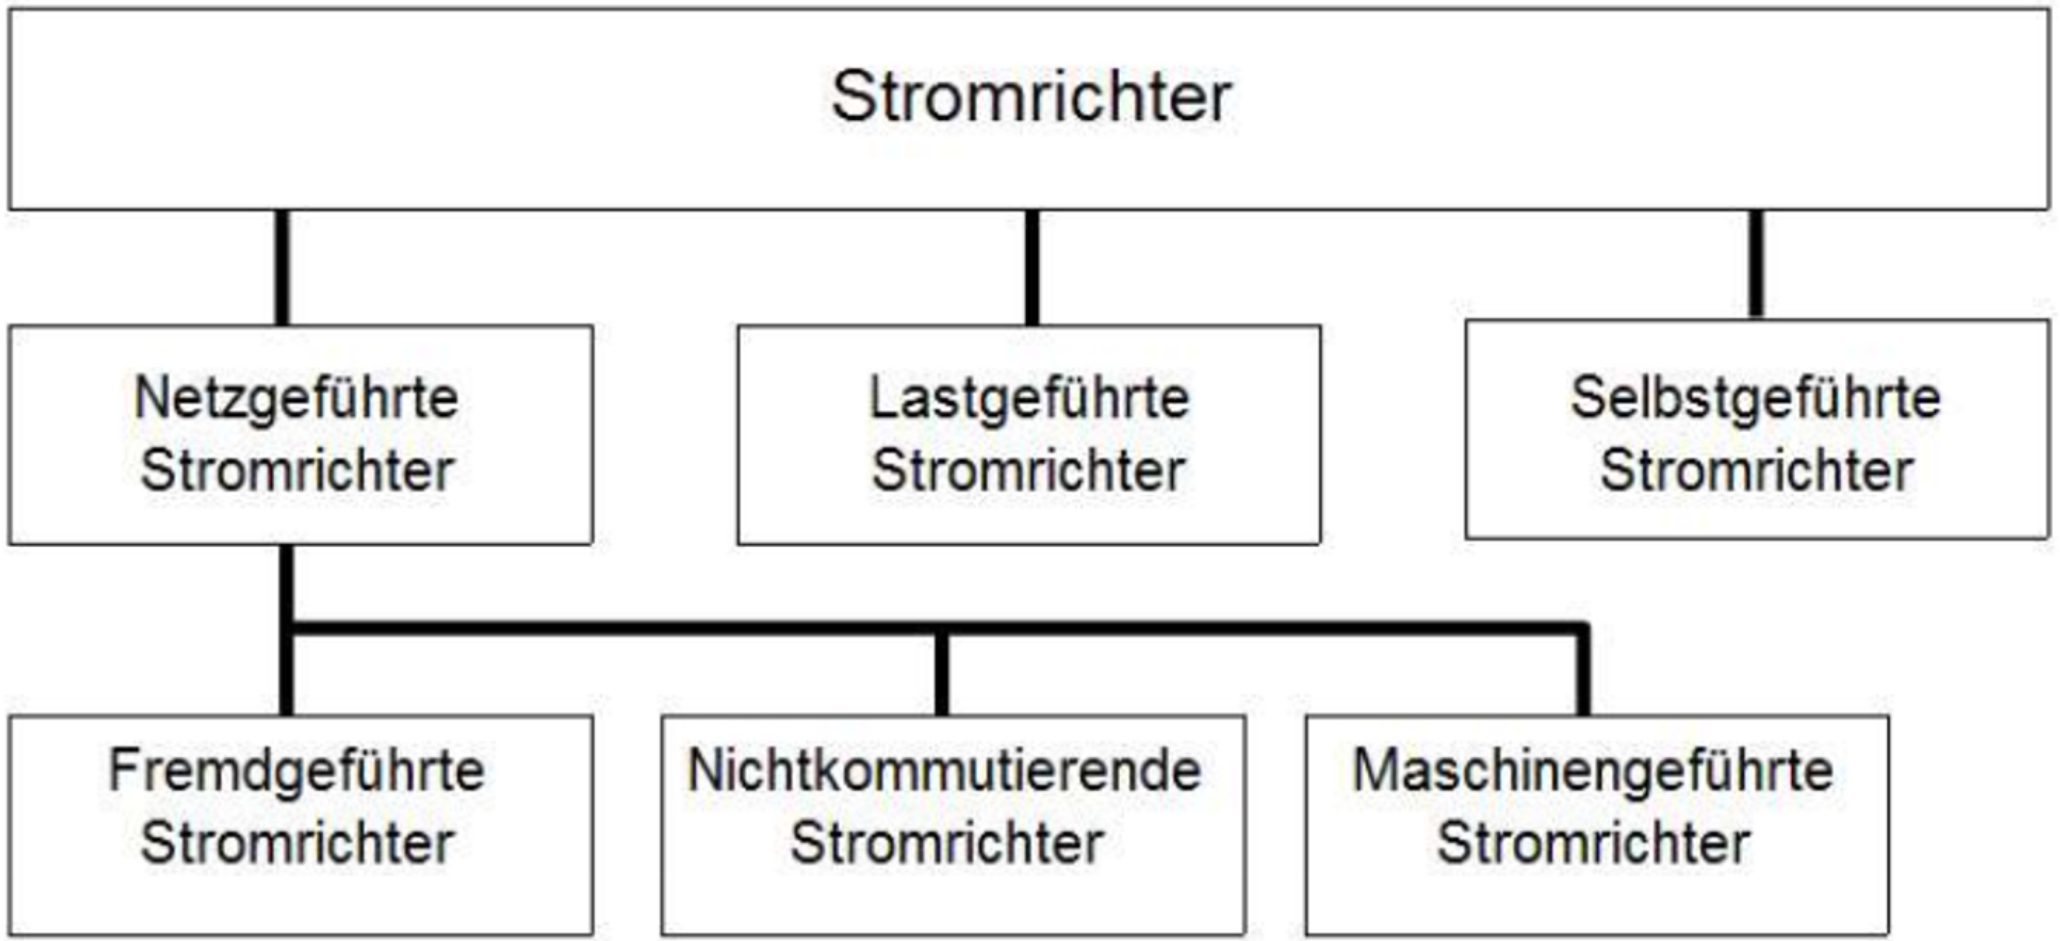
\includegraphics[width=\linewidth]{images/StromrichterKennzeichnung}\newline
\end{minipage}

\subsection{Kennzeichnung}
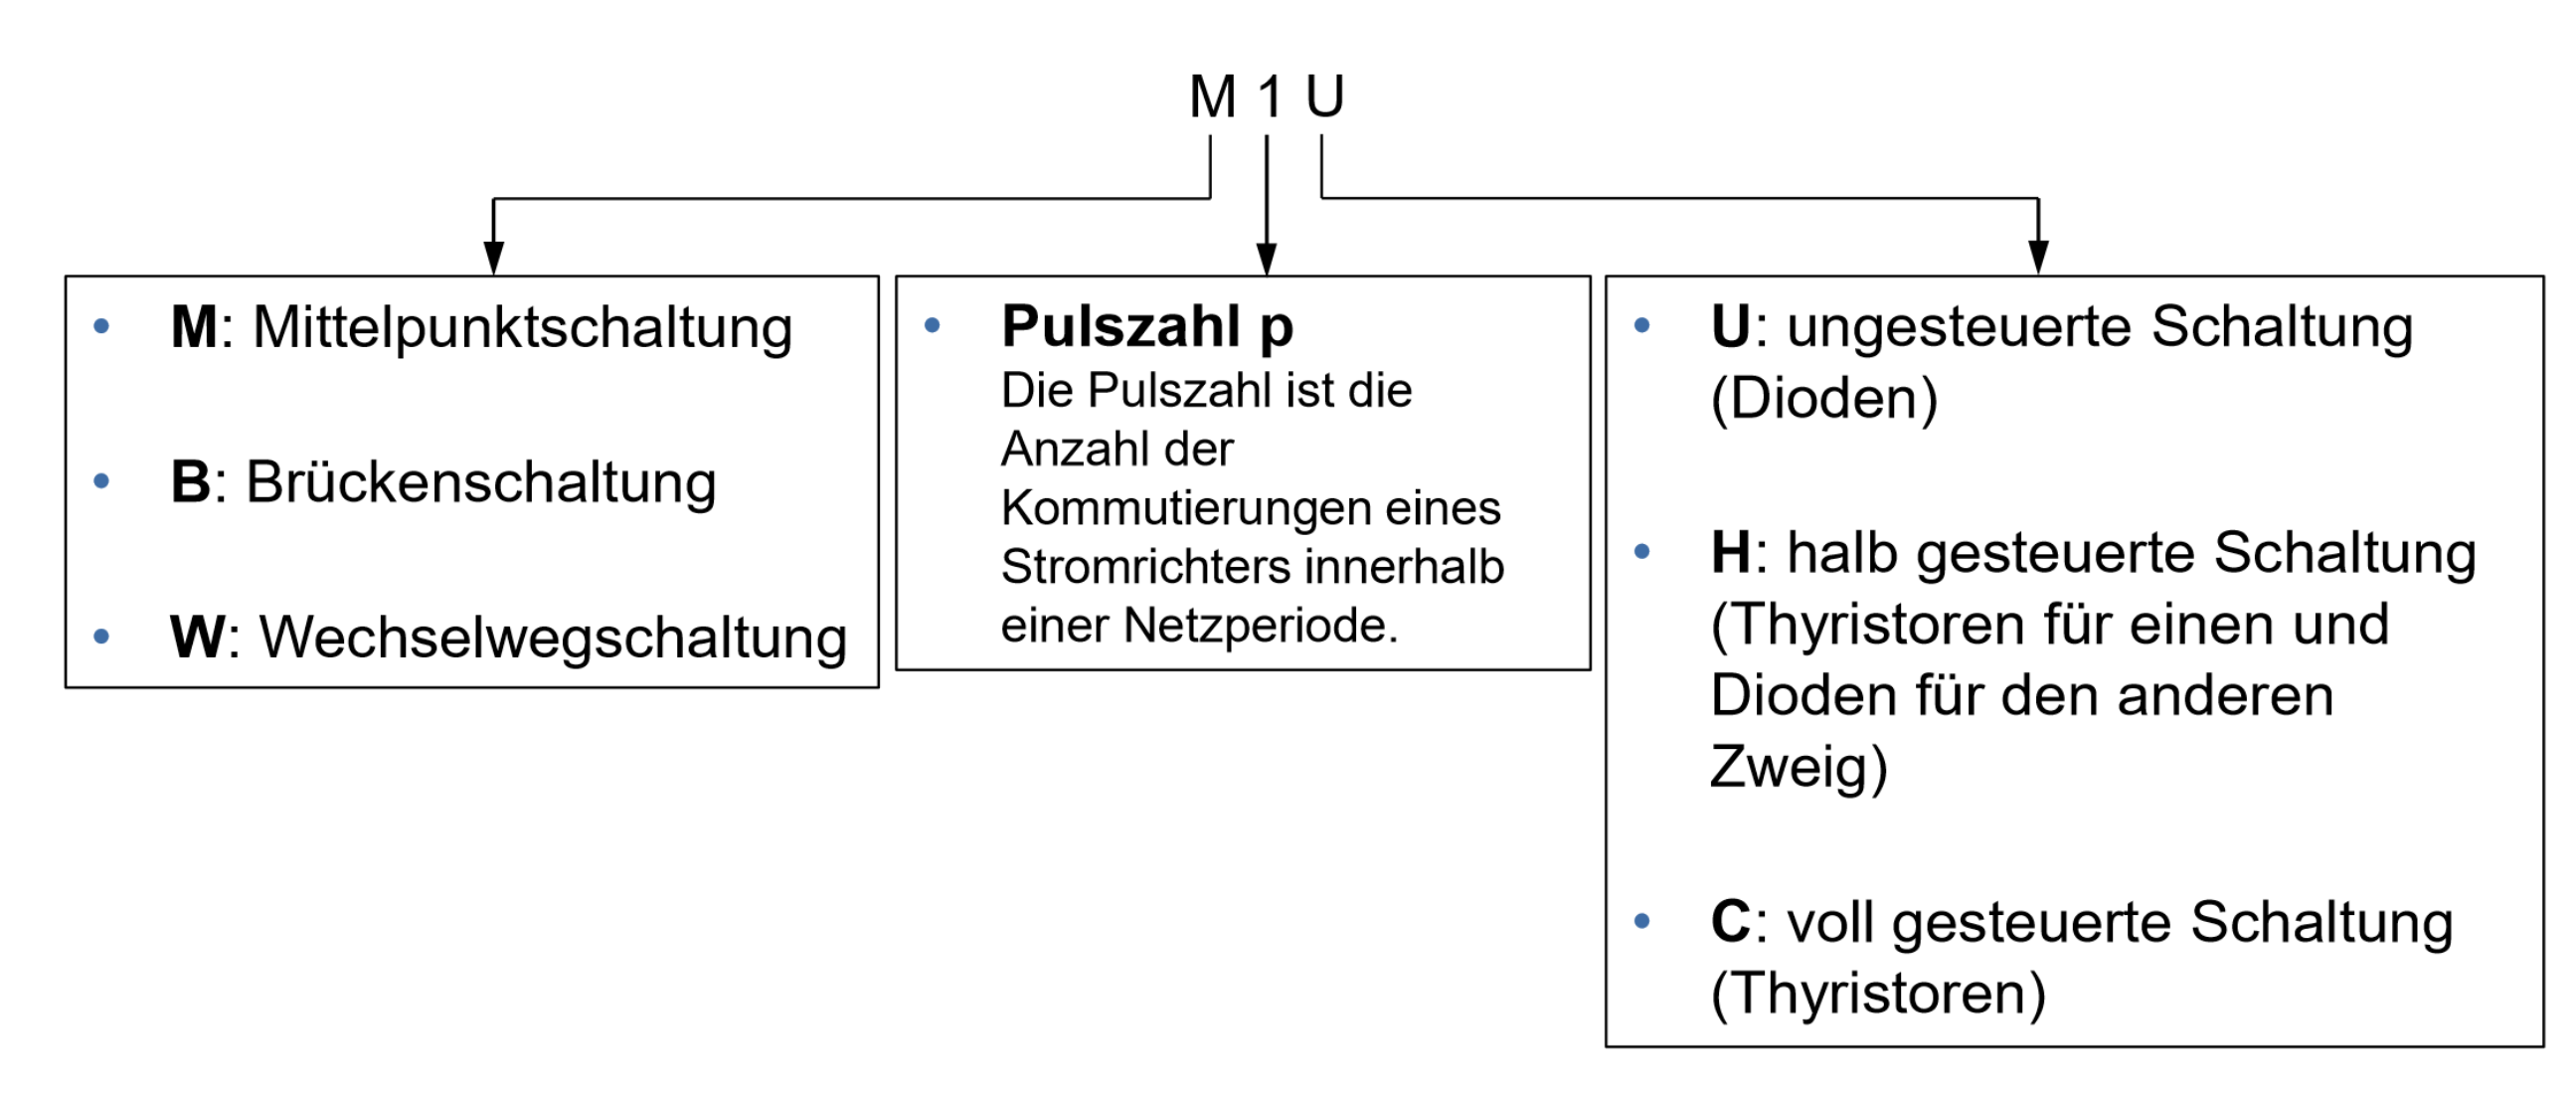
\includegraphics[width=0.8\linewidth]{images/SRKennzeichnung}\newline
\href{https://de.wikipedia.org/wiki/Gleichrichter}{Gleichrichter WIKI}

%===================================================================
\clearpage
\subsection{Ungesteuerter Gleichrichter}
\subsubsection{M1U}
\vspace{-0.5cm}
\begin{minipage}{0.4\linewidth}
    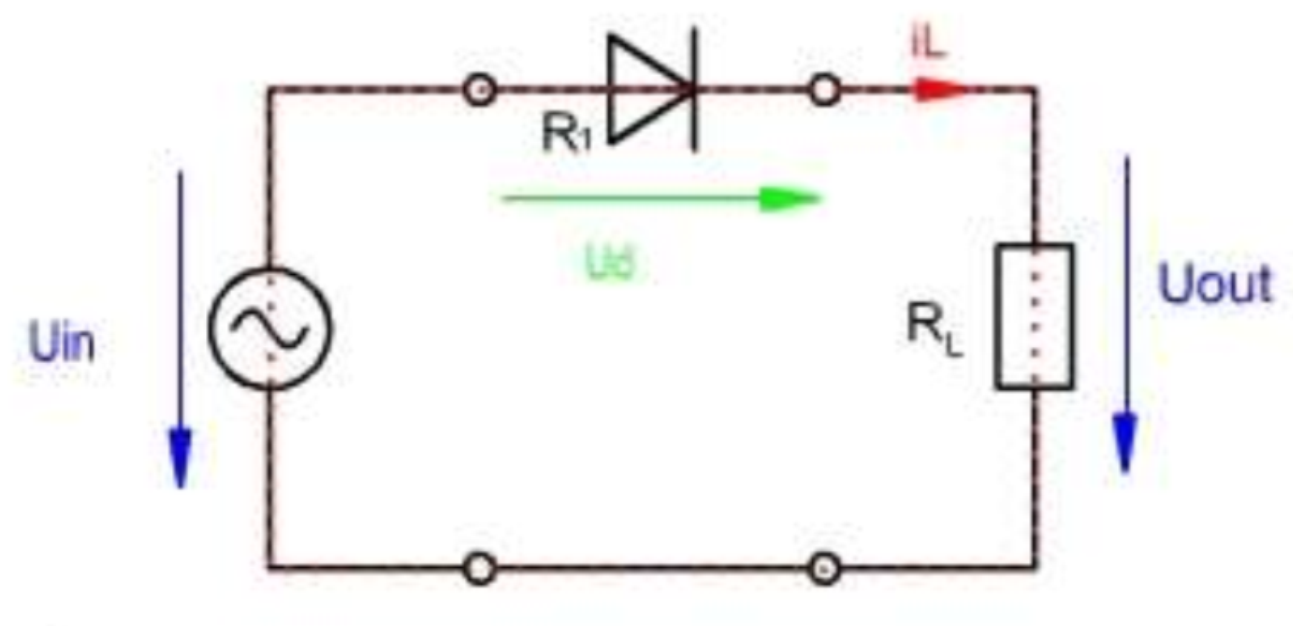
\includegraphics[width=\linewidth]{images/PrakUGM1}
\end{minipage}
\begin{minipage}{0.3\linewidth}
    \centering
   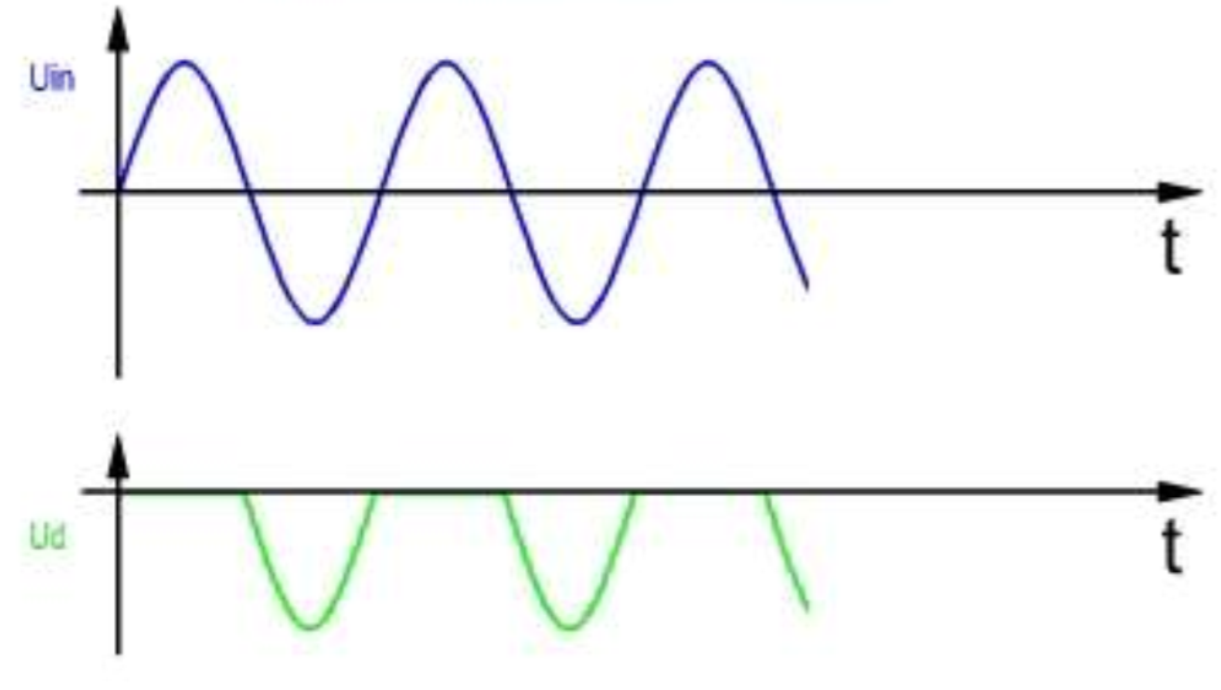
\includegraphics[width=0.7\linewidth]{images/PrakUGM1Kl1}
   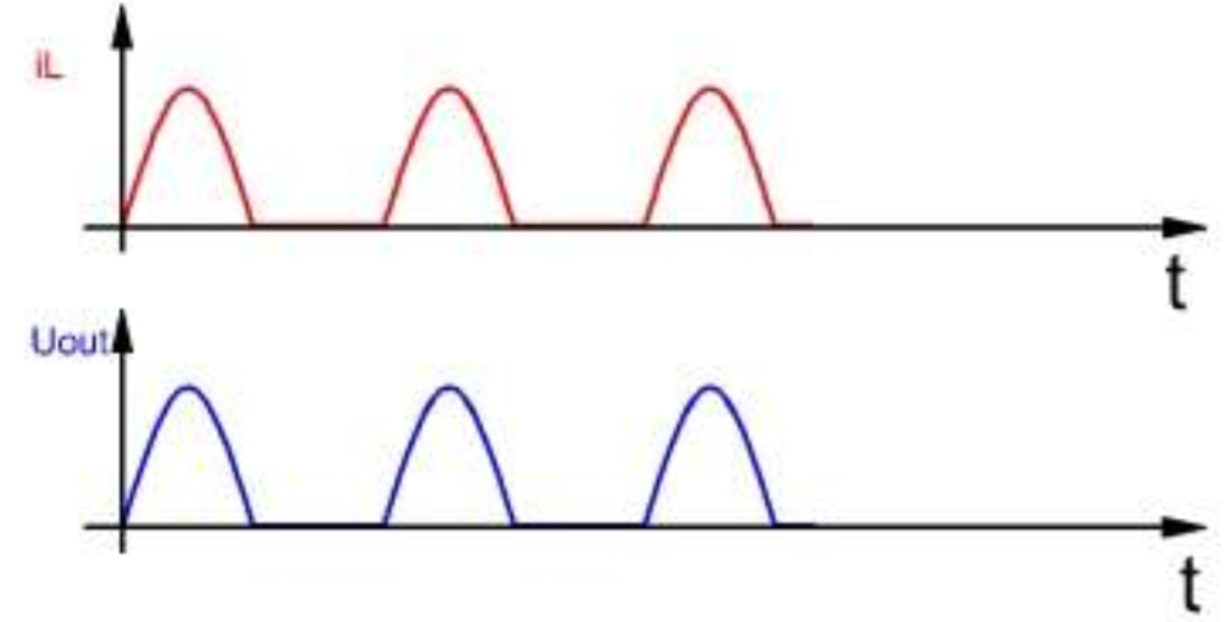
\includegraphics[width=0.7\linewidth]{images/PrakUGM1Kl2}
\end{minipage}
\begin{minipage}{0.3\linewidth}
    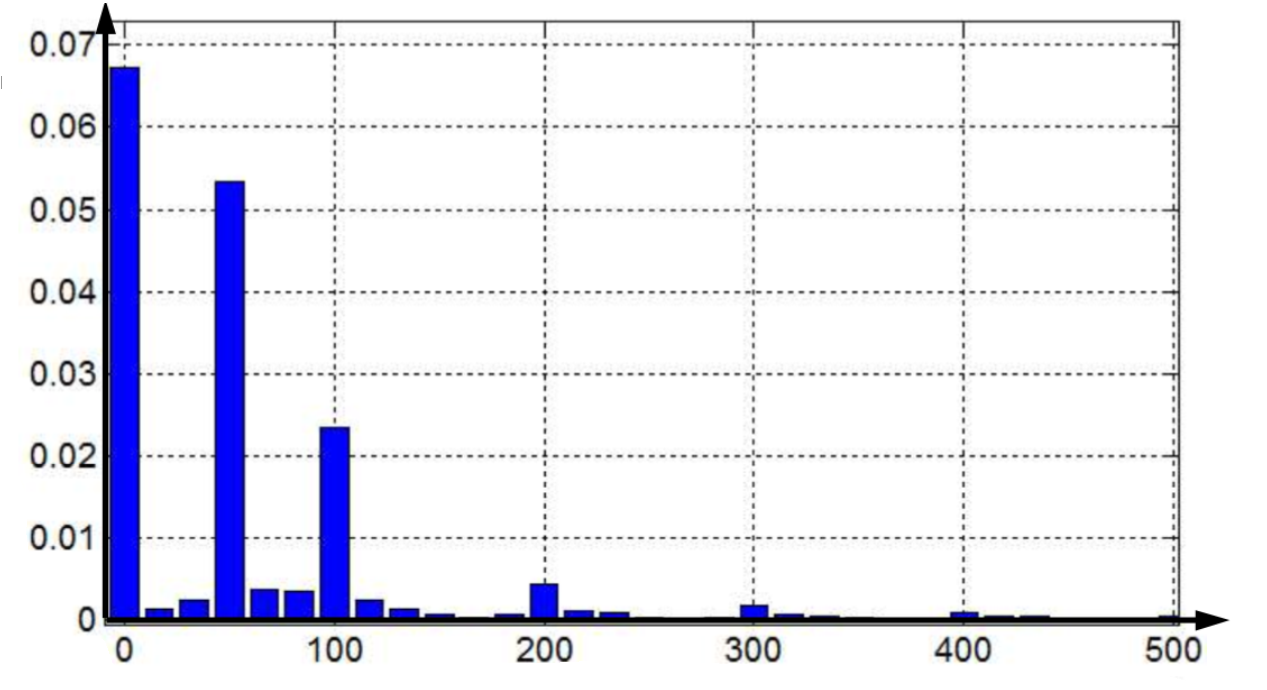
\includegraphics[width=\linewidth]{images/UGM1OW} 
\end{minipage}
\newline

%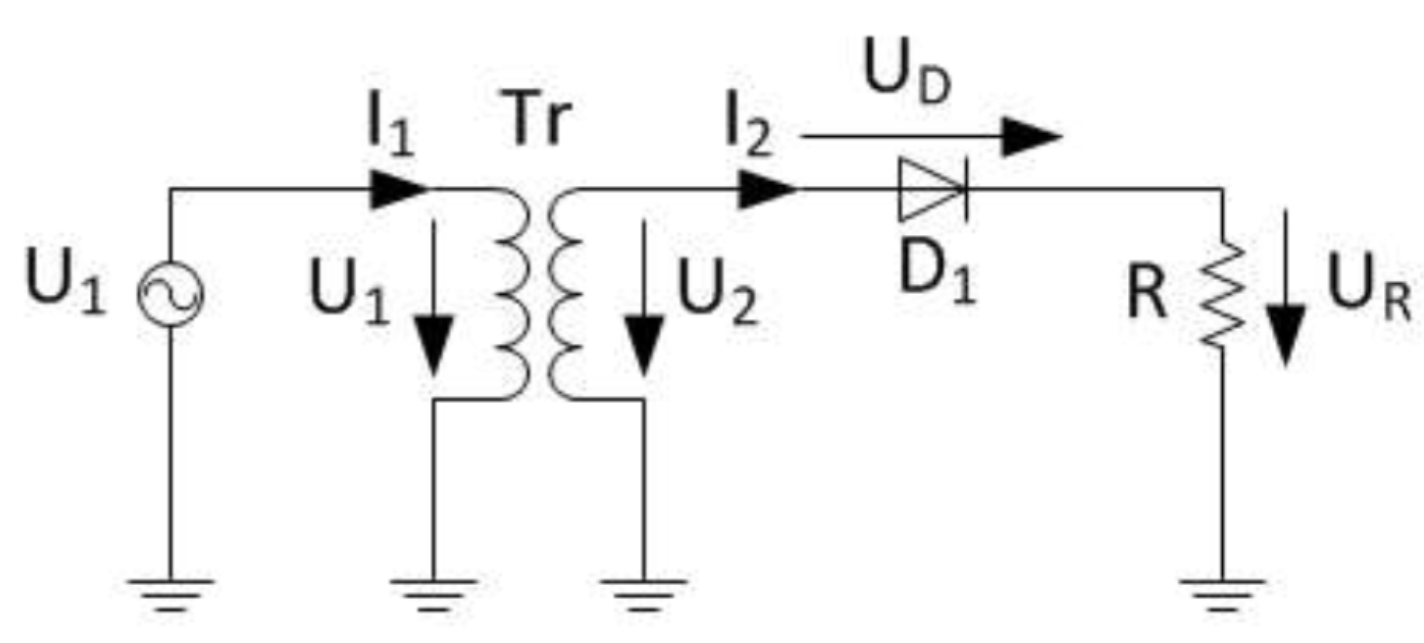
\includegraphics[width=0.4\linewidth]{images/UGRM1U}
%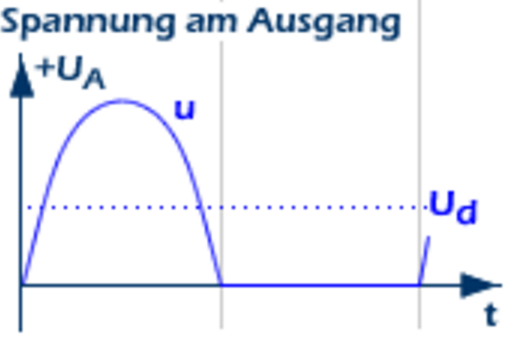
\includegraphics[width=0.2\linewidth]{images/UGRM1US} \newline
Die Diode wird als Ideal betrachtet $ \rightarrow $ keine Schwellenspannung oder Innenwiderstand
\begin{longtable}{| p{.33\textwidth} | p{.40\textwidth} | p{.25\textwidth} |} %TODO Formeln einfügen bzw anpassen
    \hline
    \textbf{Grundgleichungen}&
    \[ U_2 = U_D + U_R \]
    \[ U_R = I_2 \cdot R\]
    \[ \bar{U}_{OUT} = \dfrac{\hat{U}}{\pi}\]&\\
    \hline
    \textbf{Durchlassrichtung}\newline
    $ 0 < \omega t < \pi $&
    \vspace{-0.3cm}\[ U_2 = U_R \qquad U_D = 0 \] \vspace{-0.3cm}&\\
    \hline   
    \textbf{Sperrichtung}\newline
    $ \pi < \omega t < 2\pi $&
     \vspace{-0.3cm}\[ U_2=U_D \qquad U_R = 0 \] \vspace{-0.3cm}&\\
    \hline
    
    \textbf{Wirkleistung der Last R}&
    \[ P=\frac{1}{2\pi} \int_{0}^{2\pi} p(\alpha) d\alpha = \dfrac{U_{R\;RMS}^2}{R} \]&
    \\ \hline
    
    \textbf{Scheinleistung}&
    \[ S_2 = U_2 \cdot I_2 = U_2 \cdot I_{R RMS} \]&
    \\ \hline
        
    \textbf{Grundschwingugngsblindleistung}&
    \[ Q_2 = I_{2 1} \cdot sin(\varphi_{2 1}) = 0 \]&
    \\ \hline    
    
        
    \textbf{Verzerrungsleistung}&
    \[ Q_v = U_2 \cdot \sqrt{\sum_{k=2}^{\infty} {I_2^2}_k} = \sqrt{S_2^2 - P_2^2} \]&
    \\ \hline

\end{longtable}

%
%Leistung = Momentanleistung des Sormes x momentanleistung der Spannung\\
%Leistung = Leistung bei trafoseite messen 1harm des stroms phasenverschiebung -> u i cos(phi) fourierreihen..
%Leistung = Irav* U1harm  
\textbf{Oberwellen}\newline
\vspace{-1cm}
\begin{multicols}{3}
    \textbf{ \qquad R}\newline   
    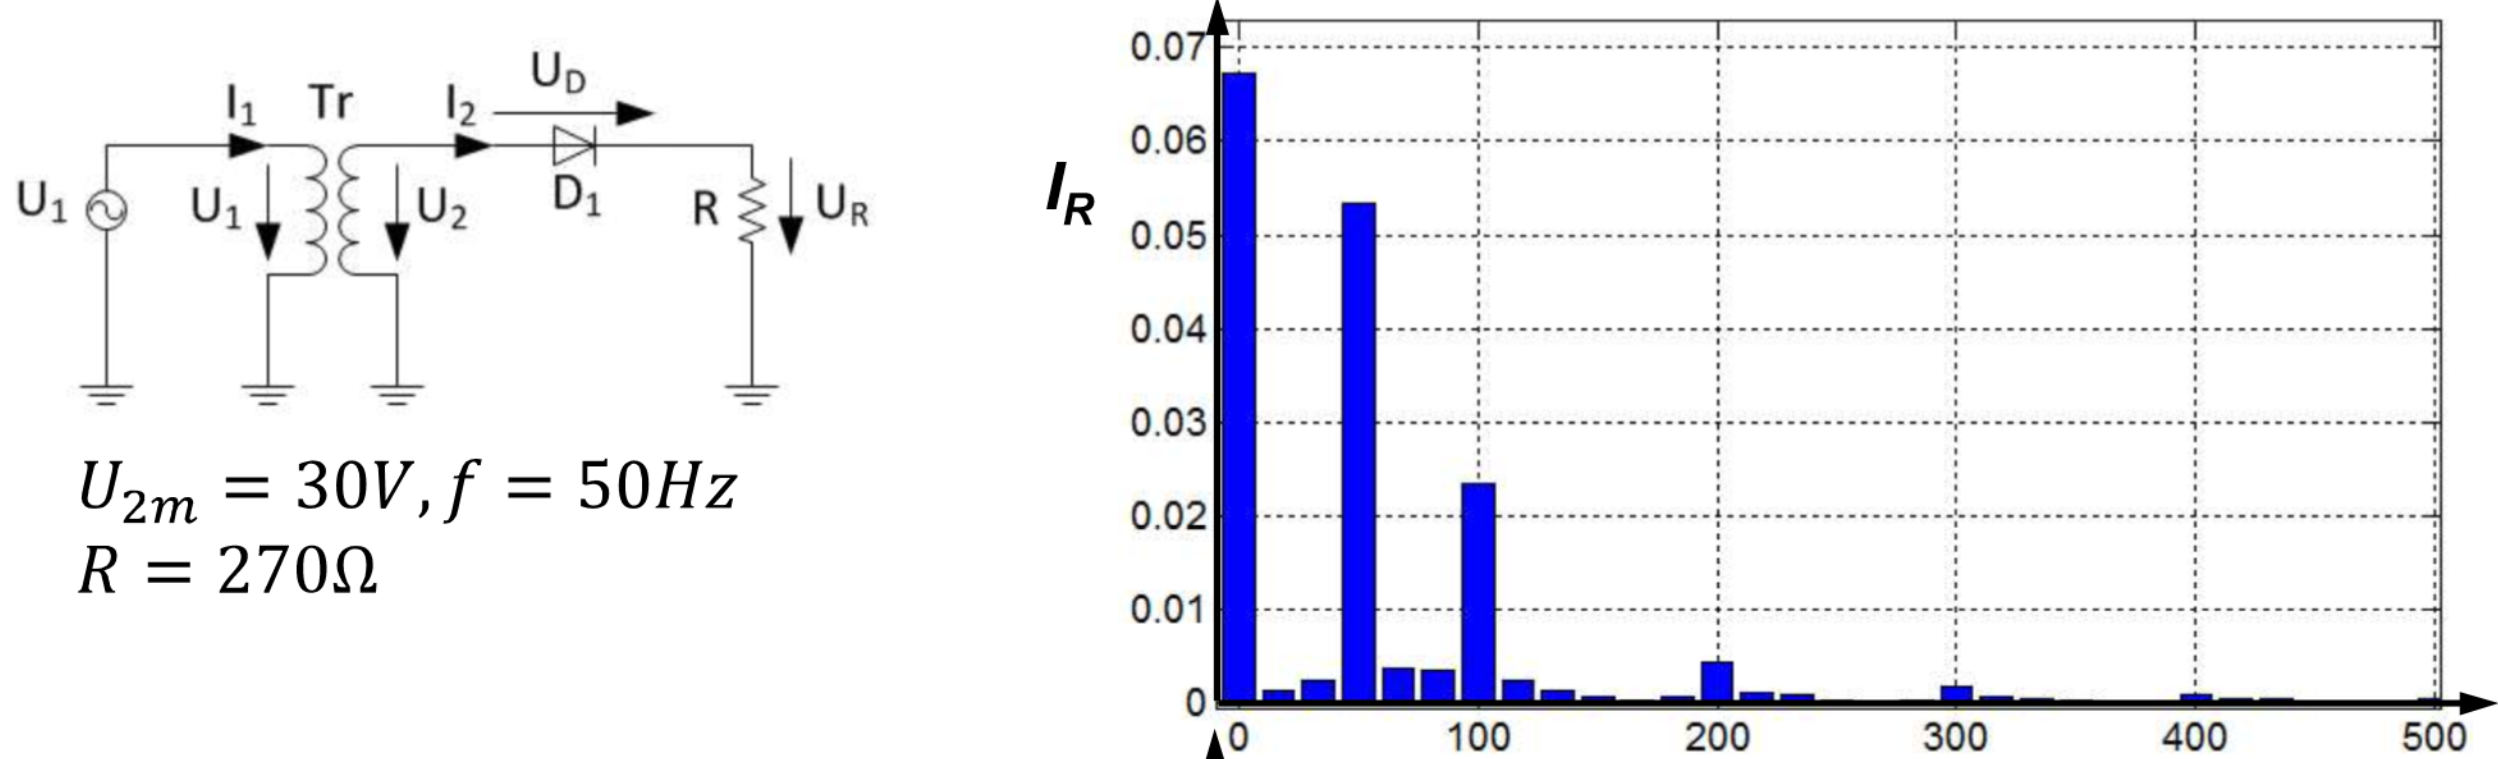
\includegraphics[width=\linewidth]{images/M1UR}   
    \textbf{\null \qquad R + L}\newline
    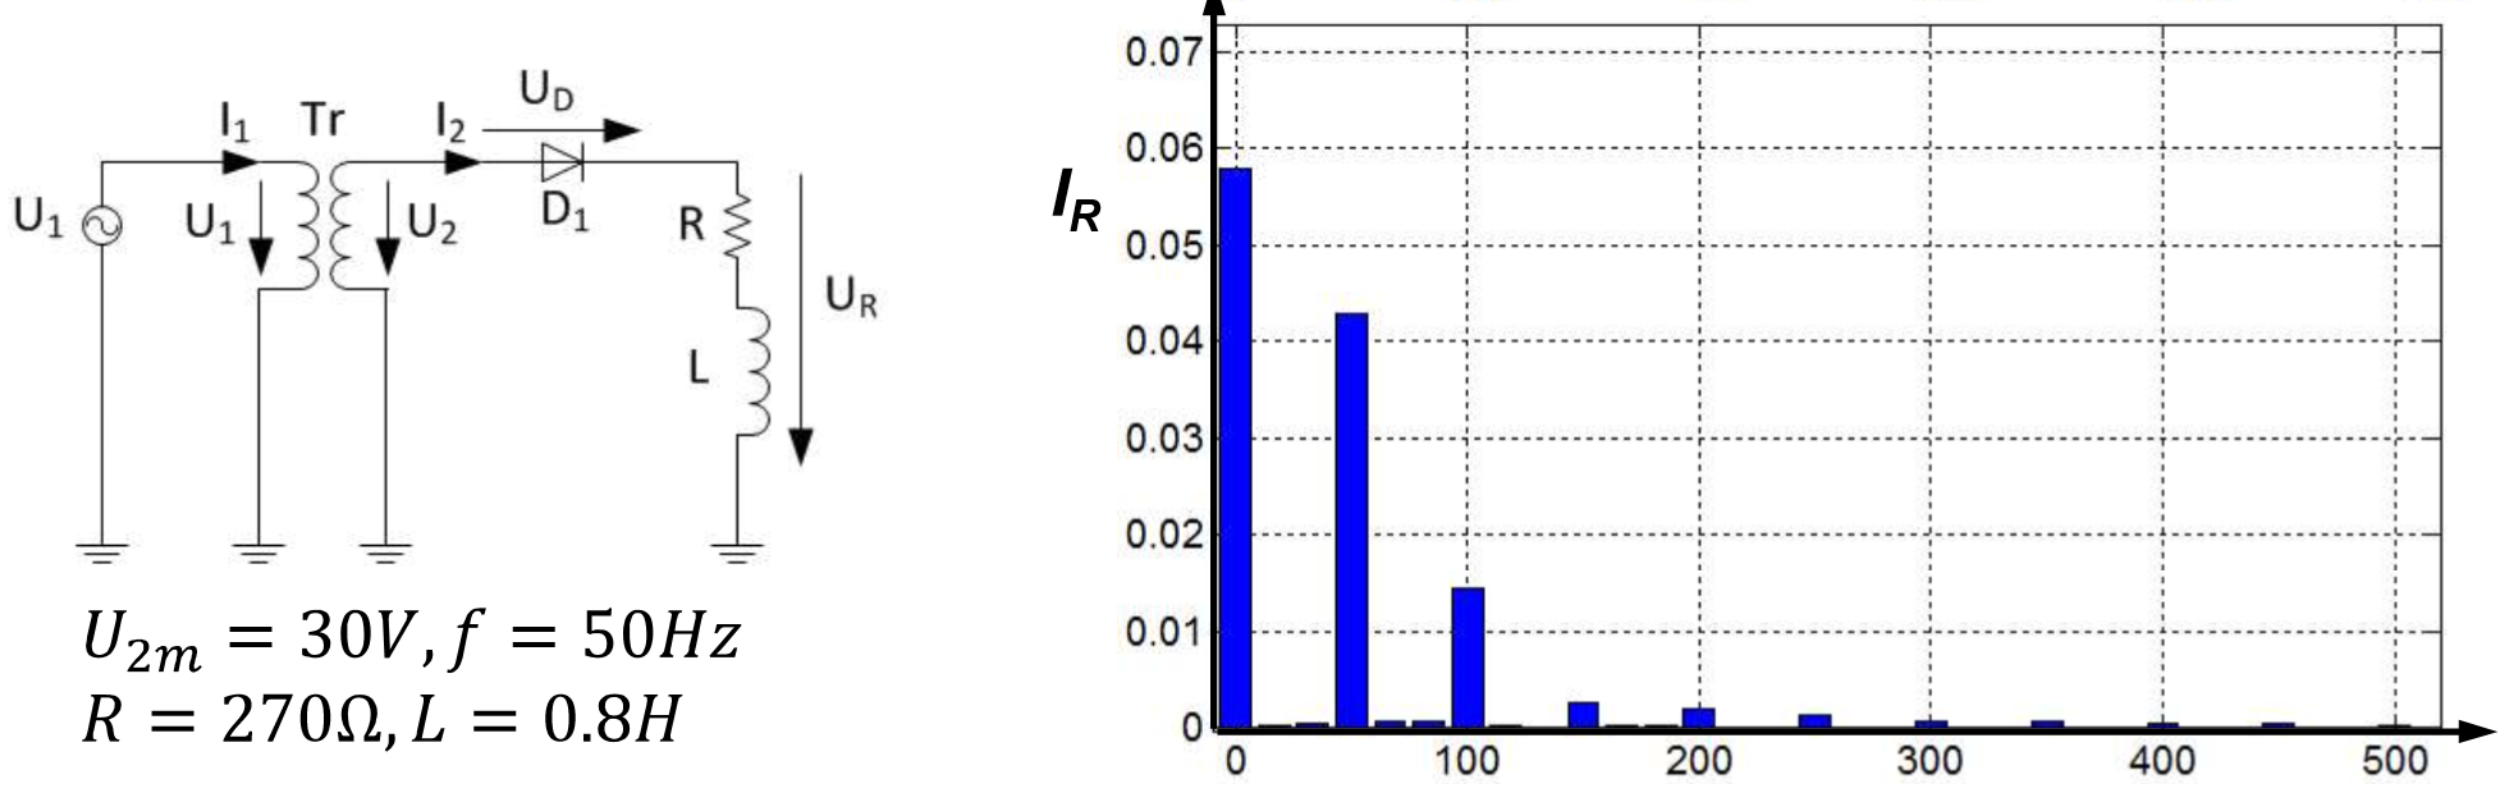
\includegraphics[width=\linewidth]{images/M1URL}
    \textbf{ \qquad R + L+ freilaufDiode}\newline
    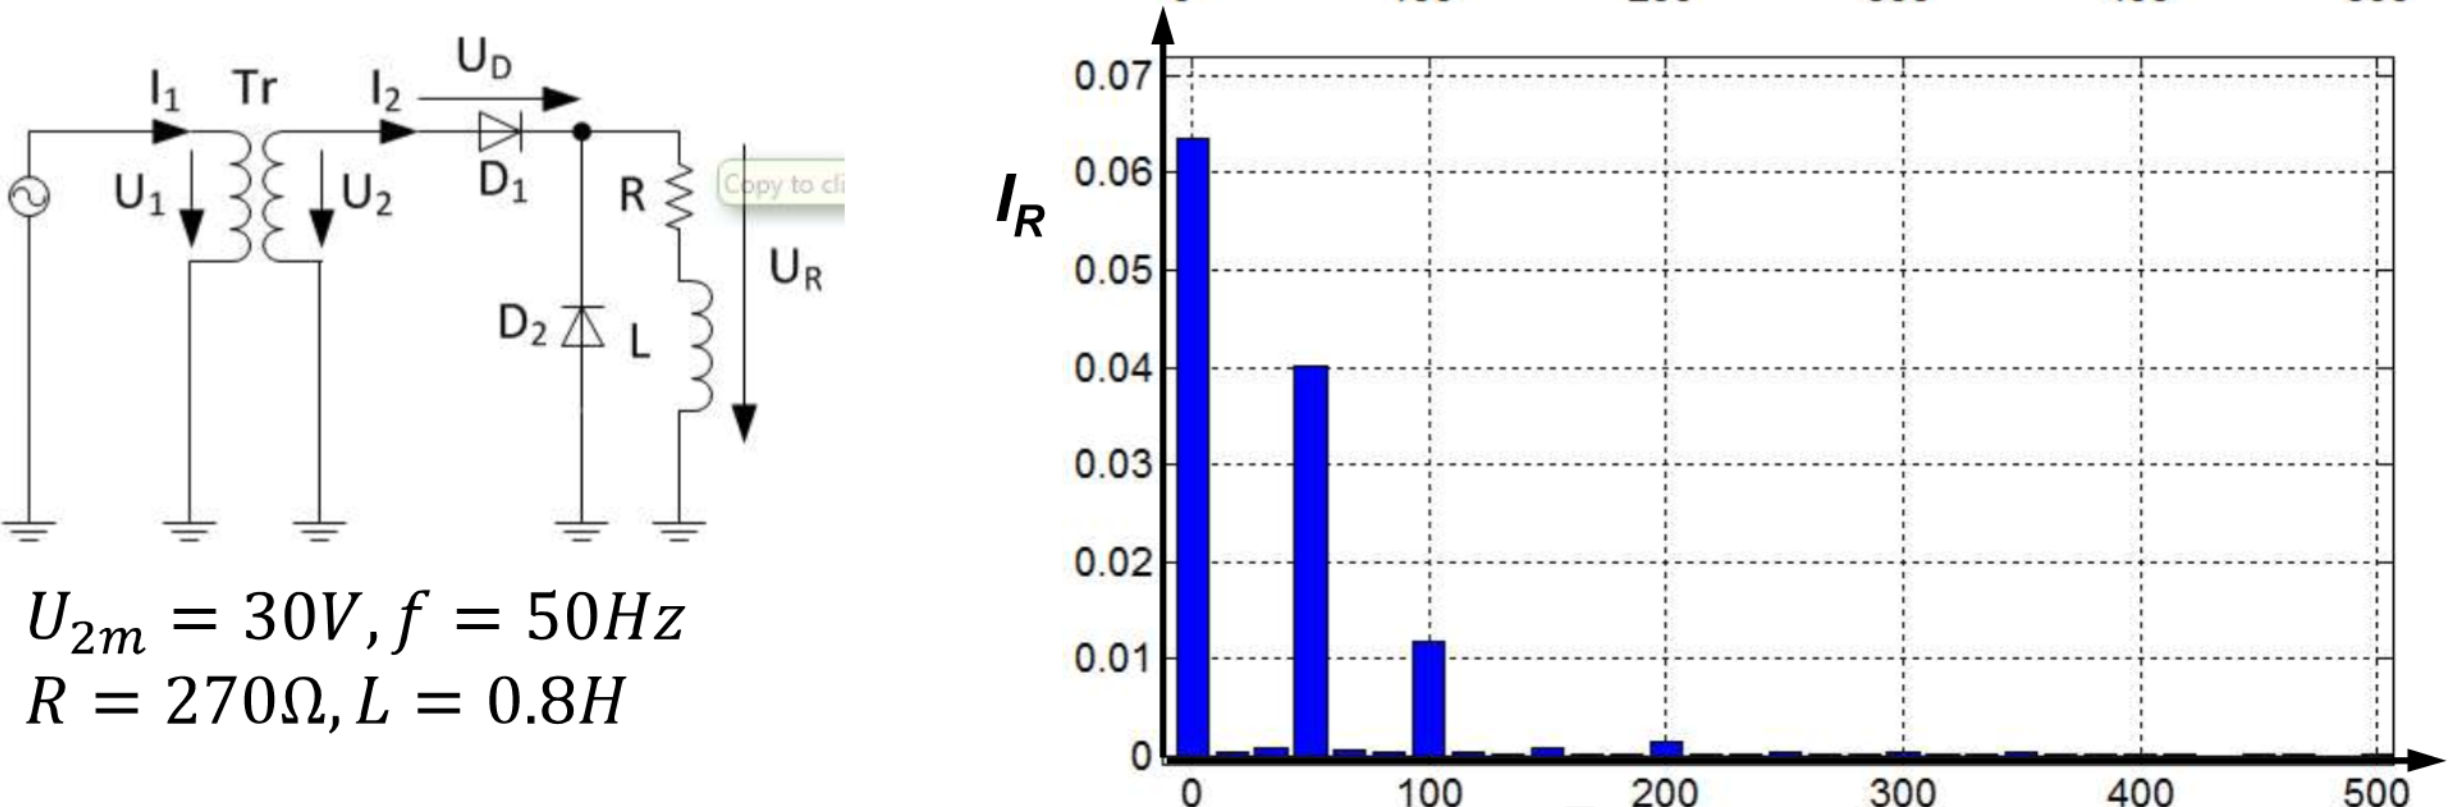
\includegraphics[width=\linewidth]{images/M1URLD}
\end{multicols}
%===================================================================
\clearpage

\subsubsection{B2U}
\begin{minipage}{0.4\textwidth}
    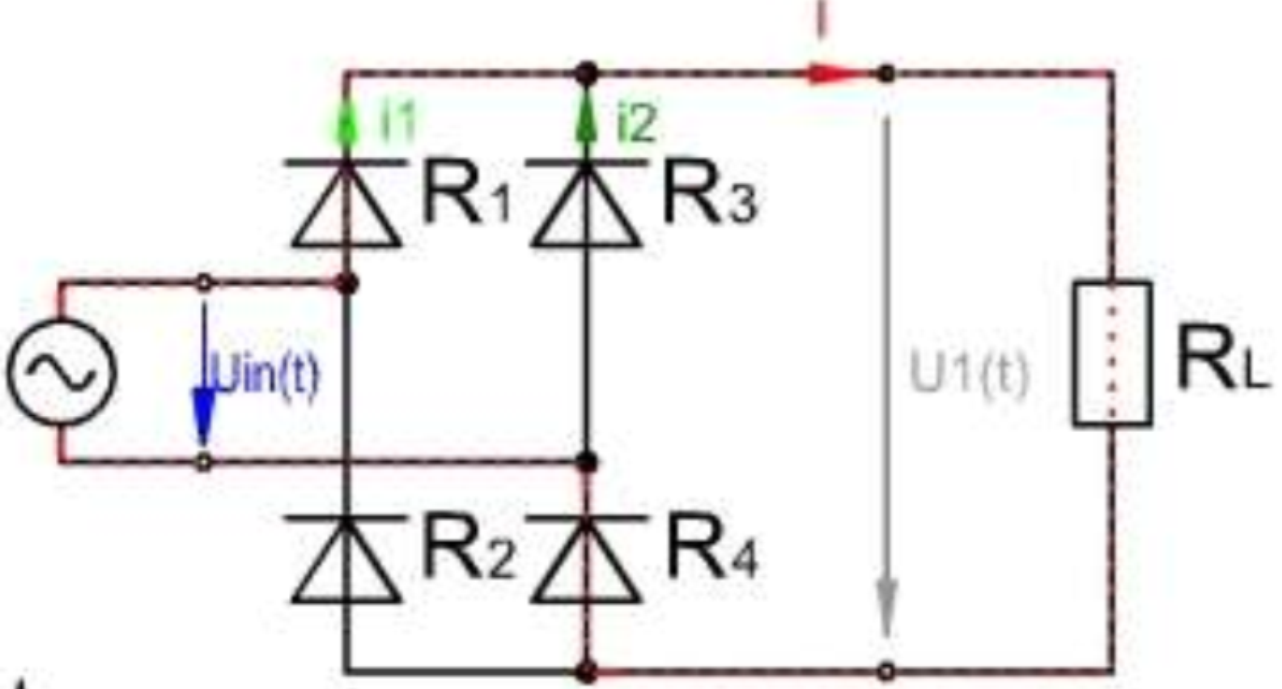
\includegraphics[width=\linewidth]{images/PrakUGB2}
\end{minipage}
\begin{minipage}{0.25\linewidth}
    \centering
    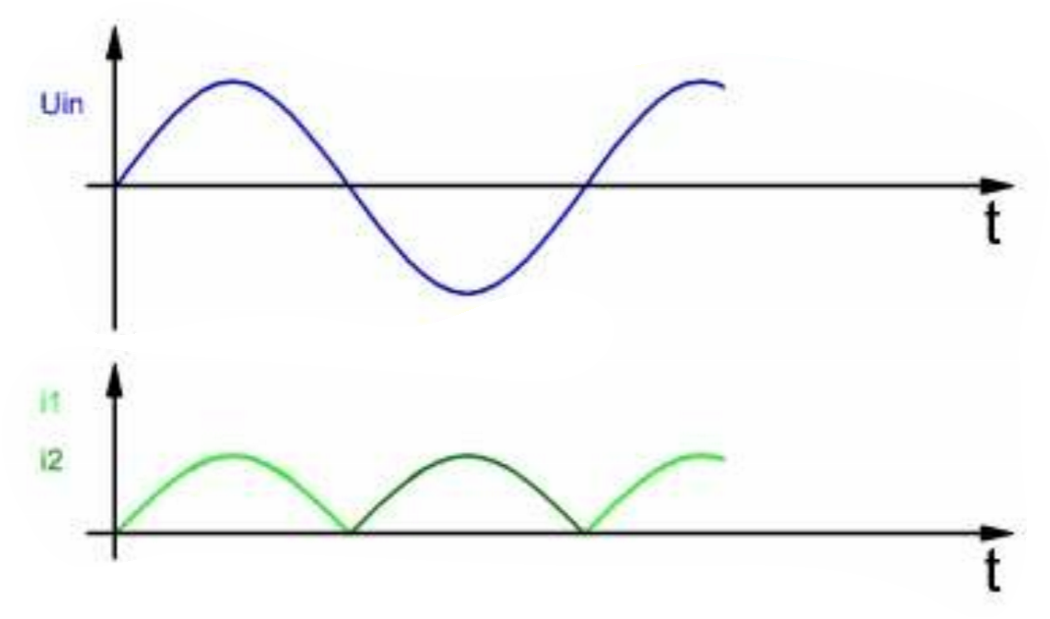
\includegraphics[width=0.9\linewidth]{images/PrakUGB2Kl1}
    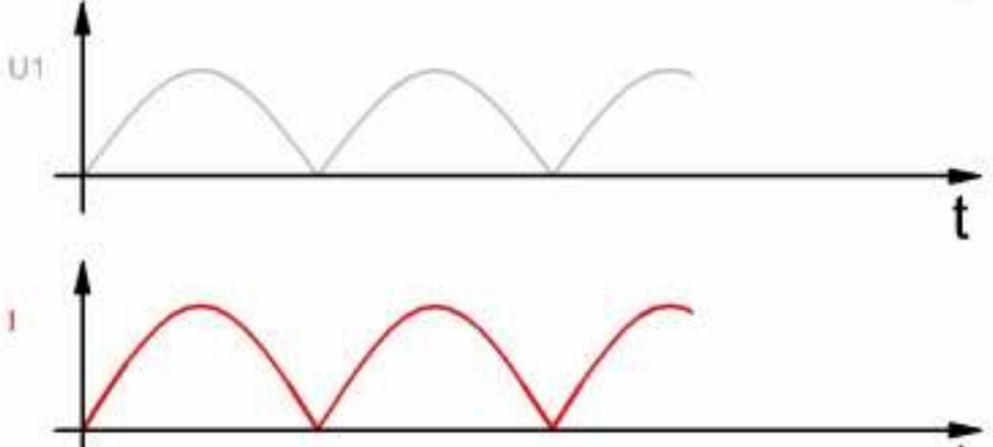
\includegraphics[width=0.9\linewidth]{images/PrakUGB2Kl2}
\end{minipage}
\begin{minipage}{0.35\linewidth}
    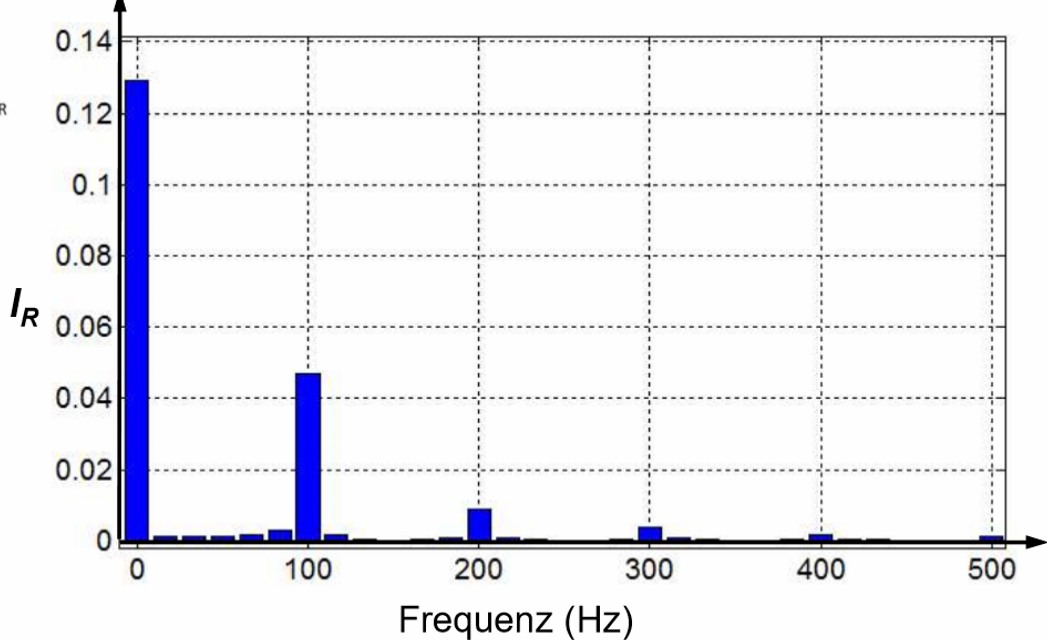
\includegraphics[width=\linewidth]{images/UGB2OW}
\end{minipage}\newline

Im gegensatz zur M1U-Schaltung wird hier die negative Netzspannung zur Gleichrichtung genutzt.\newline
Die Schaltung wird oft mit Glättungskondensator betrieben.
\begin{longtable}{| p{.33\textwidth} | p{.40\textwidth} | p{.25\textwidth} |} %TODO Formeln einfügen
    \hline
    \textbf{Grundgleichungen}&
    \[ \bar{U}_{OUT} = 2\dfrac{\hat{U}}{\pi}\]&\\
    \hline   
\end{longtable}

%===================================================================
%\clearpage

\subsubsection{B6U}
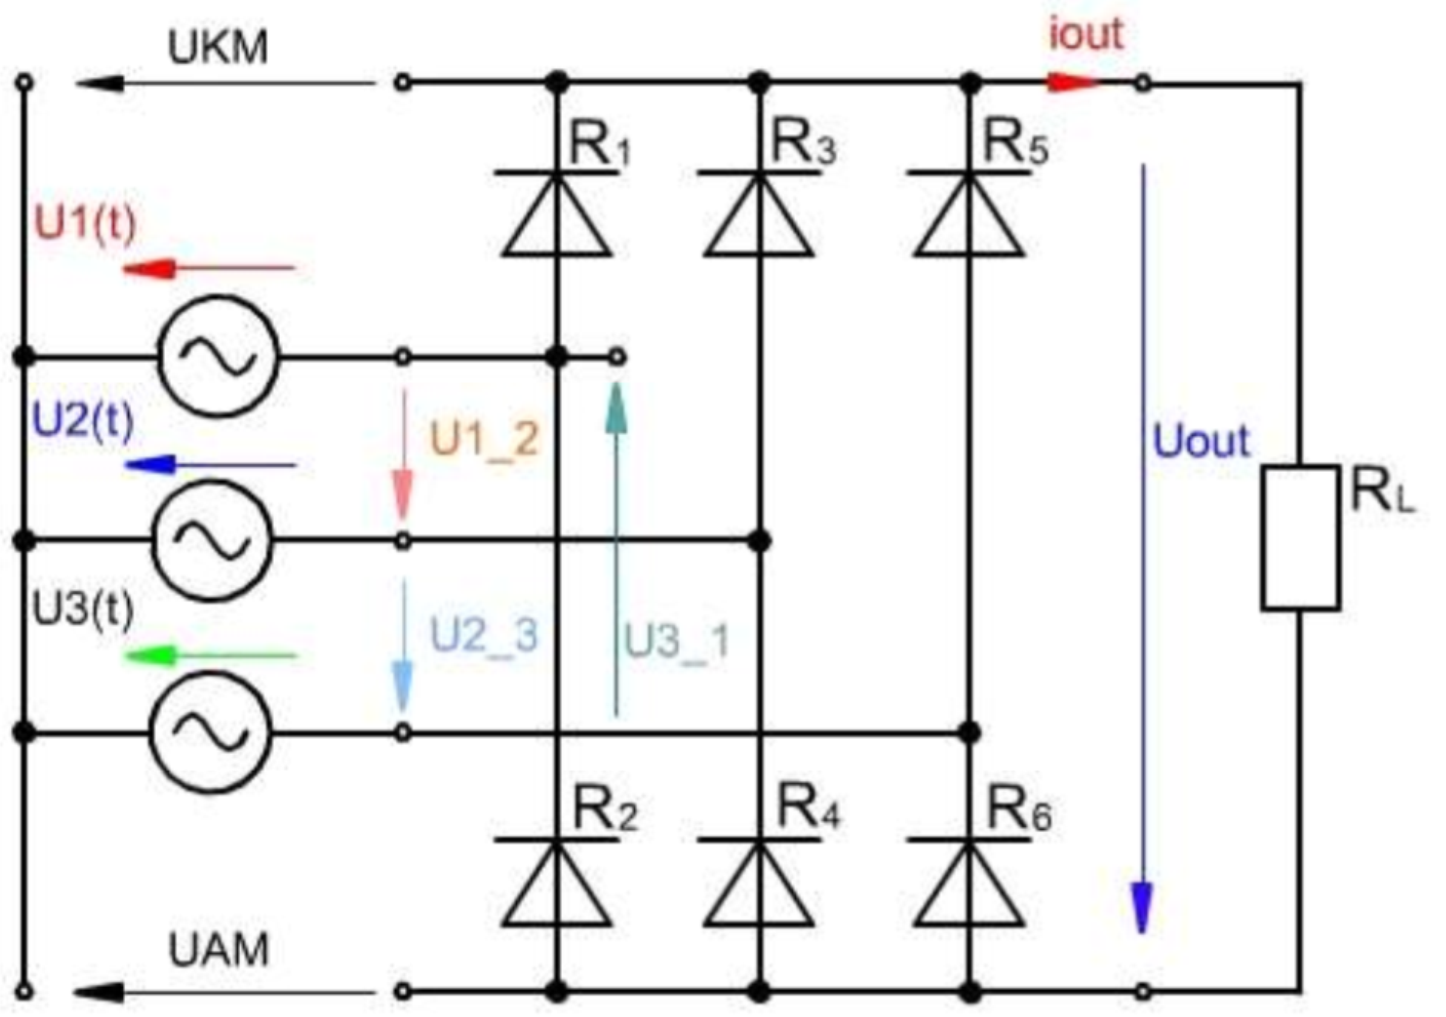
\includegraphics[width=0.3\linewidth]{images/PrakUGB6}
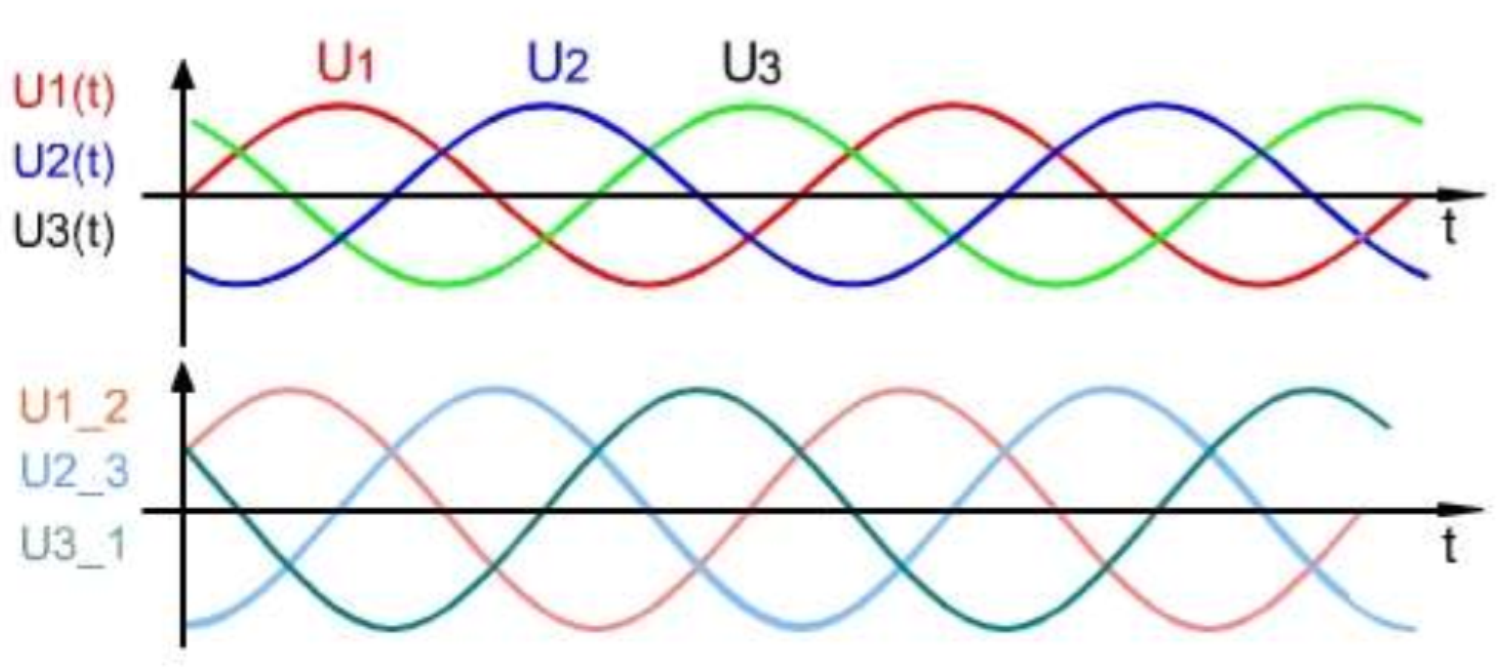
\includegraphics[width=0.3\linewidth]{images/PrakUGB6Kl1}
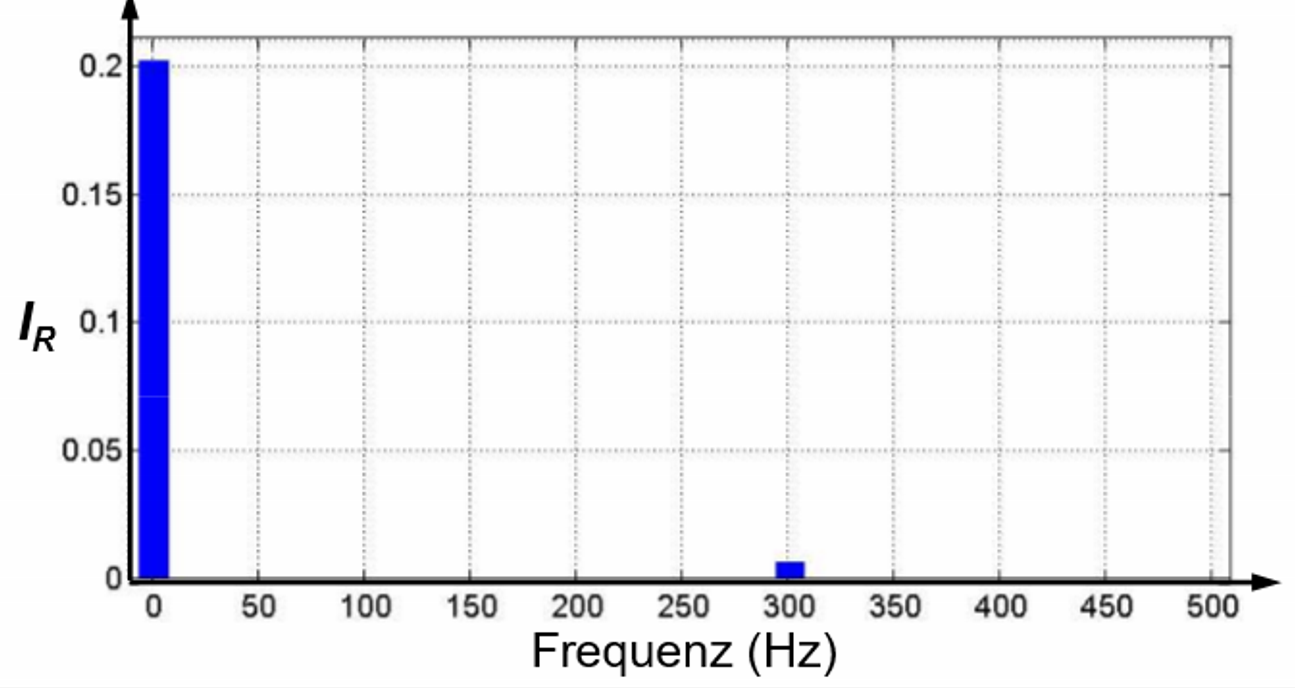
\includegraphics[width=0.3\linewidth]{images/UGB6OW}\newline
\clearpage